\section{Geometric Constraints}\label{sec:geometric}
Once we have synchronized position samples ($x_t,y_t$) from dead-reckoninig and range readings ($r_t$) from FMCW, we now need to estimate the coordinates of the points on the wall that we received reflection ($(x'_t,y'_t)$) from and those points we estimate the wall.
Since the range values are prependicular distances from the wall we get the following two geometric constraints on the values of $(x_t',y_t')$.
$$(y_t' - y_t)^2 + (x_t' - x_t)^2 = r_t^2$$.
$$\frac{y_t' - y_t}{x_t' - x_t} = \frac{-1}{m_2}$$ 

Where $m_2$ is the gradient of wall. To calculate $m_2$ we get the wall orientation with respect to the path traversed by the phone, as shown in fig XXX,  is given as $\theta = sin^{-1}(\frac{d_t}{\textbf{X}})$. Using similar triangle property $\textbf{X} = \frac{d_t \sqrt{(y_{t+1} - y_t)^2 + (x_{t+1} - x_t)^2}}{d_{t+1} - d_t}$, thus giving us 
$$\theta = sin^{-1}(\frac{d_{t+1}-d_t}{\sqrt{(y_{t+1} - y_t)^2 + (x_{t+1} - x_t)^2}})$$.

$m_2$ can now be calculated as $m_2 = tan(\theta + tan^{-1}(m_1))$, or $m_2 = tan(-\theta + tan^{-1}(m_1))$ depending on the side of the path the reflecting wall is present. Here $m_1 = \frac{y_{t+1} - y_t}{x_{t+1} - x_t}$ is the gradient of the path traversed.

Using these constraints $x_t'$ and $y_t'$ can be calculated as
$$x_t' = \pm \sqrt{r_t^2 * \frac{m_2^2}{m_2^2+1}} + x_t; $$
$$y_t' = (x_t-x_t')/m_2 + y_t$$

This would give us four set of values for $x_t'$ and $y_t'$, two on each side of the path. Using the phone orientation we know which side of the path the wall is enabling us to filter out two set of values. Among the remaining two we pick the set of values which would satisfy the following simple constraint
$$\frac{y_{t+1}' - y_t'}{x_{t+1}' - x_t'} = m_2$$
%\begin{figure}[hbt]
%  %\vspace{-0.15in}
%\centering{
%\subfigure[]{
%    \fbox{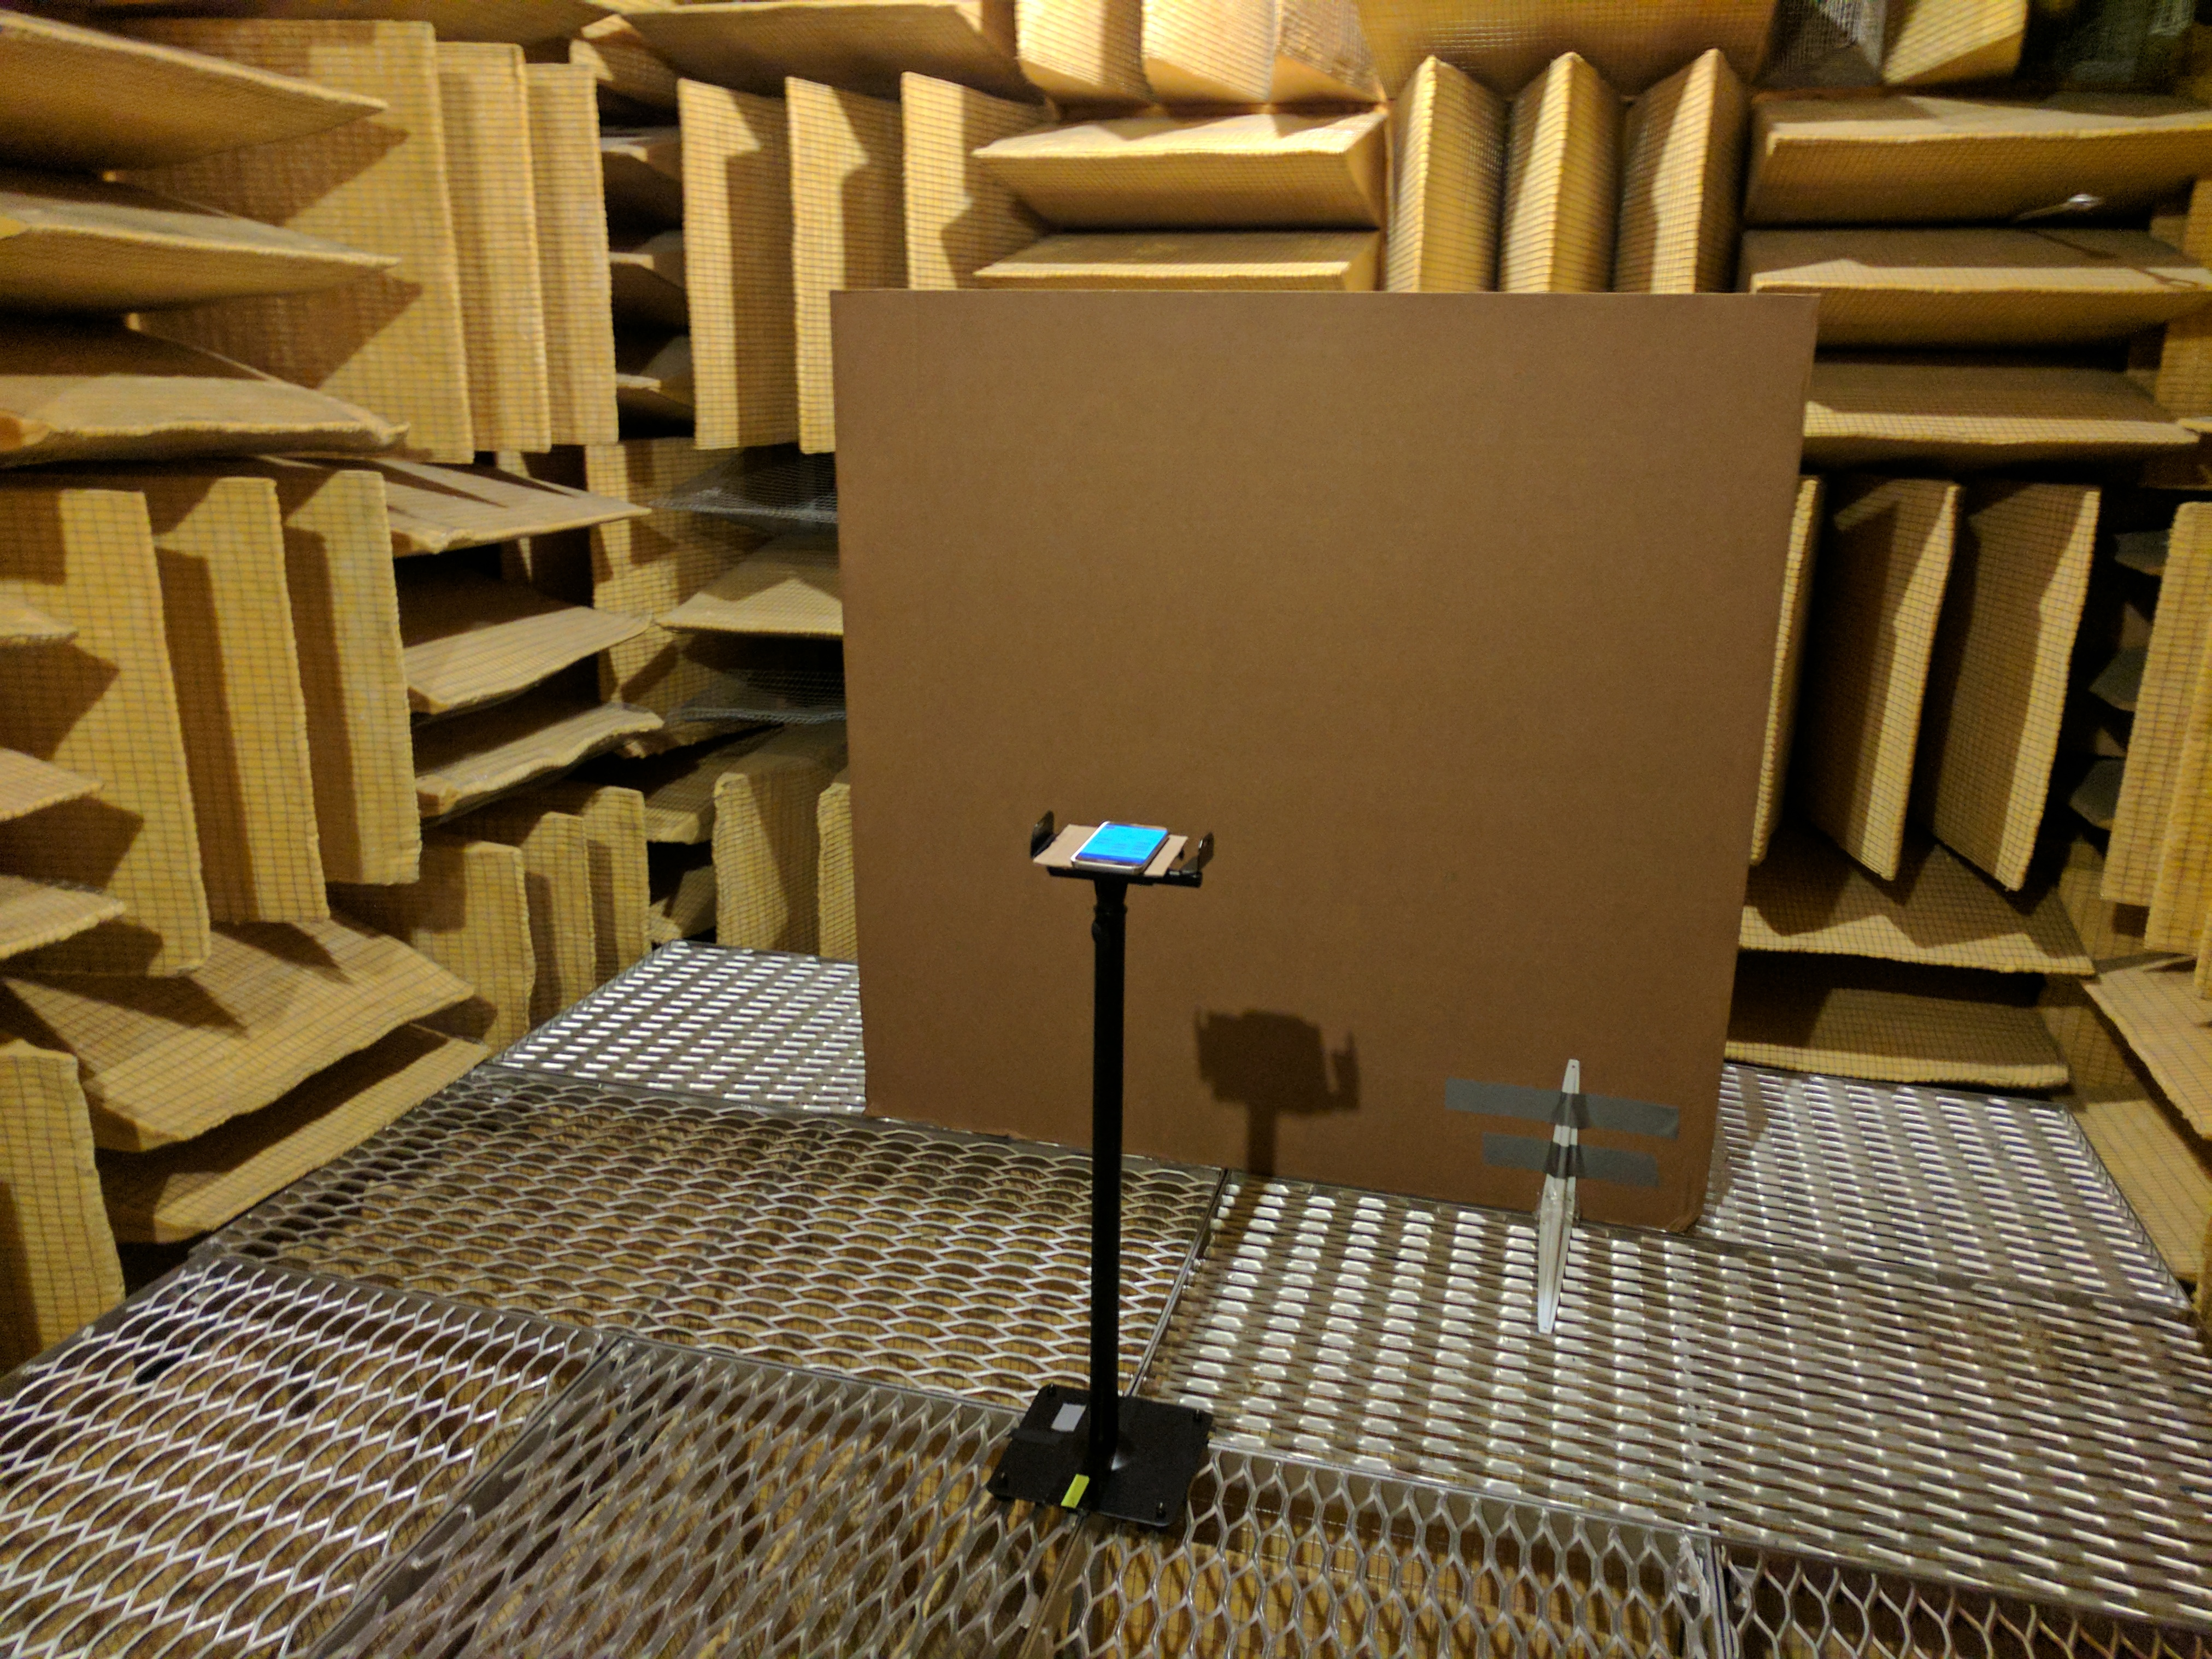
\includegraphics[width=0.40\columnwidth, %keepaspectratio]{figs/anechoic_experiment.jpg}}
%    \label{fig:anechoic}
%}
